\documentclass[tikz,border=10pt]{article}
\newcommand{\course}{Pre-Calculus}
\usepackage[margin=1.5in]{geometry}
\newcommand{\instructor}{Athan Zhang \& Jeffrey Chen}
\usepackage{amsmath}
\usepackage{pgfplots}
\pgfplotsset{width=10cm, compat=1.9}
\usepackage[inline]{enumitem}

\usepgfplotslibrary{external}
\tikzexternalize
\pgfplotsset{compat=1.12}


% Document Body
\begin{document}

% Title
\begin{center}
\textbf{\Huge Problem Set 01} % Replace "#" with the problem set number
\end{center}

% Course and Instructor Information
\begin{flushleft}
\emph{Course:} \course \\
\emph{Instructors:} \instructor \\
\end{flushleft}

% Problem 1
\section*{Problem 1}

Write each set of numbers using interval notation: 

\begin{enumerate}
    \item $x \geq 21$
    \item $x < 7$
    \item $-3 \leq x < 10$
    \item $x \geq 3$ or $x \leq -82$
    \item $x > 71$ or $x \leq 0$
\end{enumerate}

% Problem 2
\section*{Problem 2}

Describe the domain and range of the following functions:

\begin{enumerate}
    \item $f(x) = x$
    \item $f(x) = \frac{x-2}{x^{2} - 4}$
    \item $f(x) = \frac{1}{x+3}$
    \item $f(x) = \frac{(x-1)^{3/2}}{x-1}$
\end{enumerate}

% Problem 3
\section*{Problem 3}

Determine if the following functions are continuous at the given point. If not, describe the type of discontinuity. State what rules of the continuity test are violated, if any.

\begin{enumerate}
    \item $f(x) = 2x^{2} -3x -1$; at $x = 2$
    \item $f(x) = \frac{1}{x^{2}}$; at $x = 0$
    \item $f(x) = \begin{cases}
         5x + 4 & \text{if } x > 2, \\
         2 - x & \text{if } x \leq 2.
       \end{cases}$; at $x = 2$
\end{enumerate}

% Problem 4
\section*{Problem 4}
Using the graphs of the following function, give the intervals on which the function is increasing, decreasing, or constant.

\begin{center}
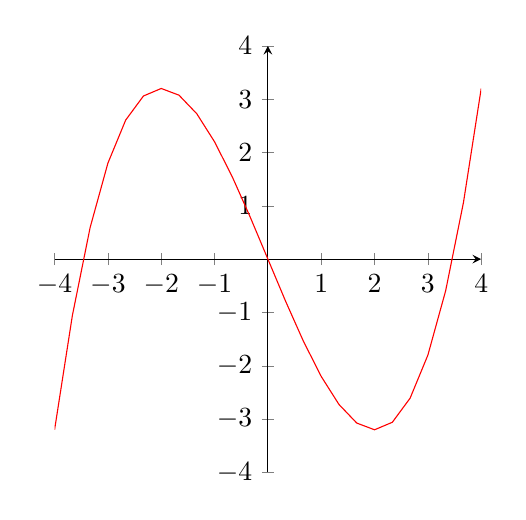
\begin{tikzpicture}
\begin{axis}[
    axis lines=middle, width=7cm, height=7cm, ymin=-4, ymax=4, ytick={-4, -3, -2, -1, 1, 2, 3, 4}, xmin=-4, xmax=4, xtick={-4, -3, -2, -1, 1, 2, 3, 4}
]
\addplot[domain=-4:4, color=red]{0.2*(x^3-12*x)};
\end{axis}
\end{tikzpicture}
\end{center}

% Problem 5
\section*{Problem 5}

Find the average rate of change of each function in the given interval

\begin{enumerate}
    \item $f(x) = 3x^{2} - 8x + 2$; $[4,6]$
    \item $f(x) = \frac{1}{x}$; $[3,5]$
    \item $f(x) = \sqrt{x + 8}$; $[-4, 4]$
\end{enumerate}

% Problem 6
\section*{Problem 6}

Find $(f + g)(x)$, $(f - g)(x)$, $(f\cdot g)(x)$, and $(\frac{f}{g})(x)$ for the follwoing. State the domain of each new function.

\begin{align*}
    f(x) &= x^2 + 4 \\
    g(x) &= \sqrt{x}
\end{align*}

% Problem 7
\section*{Problem 7}

Find $(f \circ g)(x)$

\begin{align*}
    f(x) &= \frac{2}{x - 3} \\
    g(x) &= x^{2} + 6
\end{align*}

% Problem 8
\section*{Problem 8}

For each $f(x)$ (red), use the graph to find the equation of $g(x)$ (blue).

\begin{center}
\begin{enumerate}
    \item
    \begin{center}
    $f(x) = \frac{1}{x}$
    \newline
    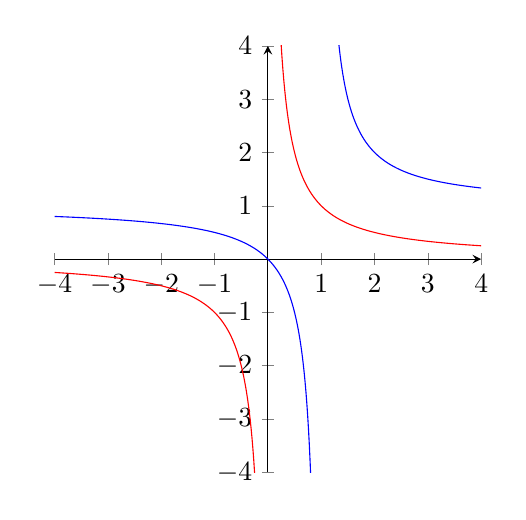
\begin{tikzpicture}
    \begin{axis}[
        axis lines=middle, width=7cm, height=7cm, ymin=-4, ymax=4, ytick={-4, -3, -2, -1, 1, 2, 3, 4}, xmin=-4, xmax=4, xtick={-4, -3, -2, -1, 1, 2, 3, 4}, samples=500, restrict y to domain=-30:30
    ]
    \addplot[domain=-4:4, color=red]{1/x};
    \addplot[domain=-4:4, color=blue]{(1/(x-1))+1};
    \end{axis}
    \end{tikzpicture}
    \end{center}

    \item
    \begin{center}
    $f(x) = x^4$
    \newline
    \begin{tikzpicture}
    \begin{axis}[
        axis lines=middle, width=7cm, height=7cm, ymin=-4, ymax=4, ytick={-4, -3, -2, -1, 1, 2, 3, 4}, xmin=-4, xmax=4, xtick={-4, -3, -2, -1, 1, 2, 3, 4}
    ]
    \addplot[domain=-4:4, color=red]{x^4};
    \addplot[domain=-4:4, color=blue]{0.5*(x+1)^4};
    \end{axis}
    \end{tikzpicture}
    \end{center}
    % \item
    % \begin{tikzpicture}
    % \begin{axis}[
    %     axis lines=middle, width=7cm, height=7cm, ymin=-4, ymax=4, ytick={-4, -3, -2, -1, 1, 2, 3, 4}, xmin=-4, xmax=4, xtick={-4, -3, -2, -1, 1, 2, 3, 4}
    % ]
    % \addplot[domain=-4:4, color=red]{x^{3}};
    % \addplot[domain=-8:4, color=blue]{(x+2)^{3}};
    % \end{axis}
    % \end{tikzpicture}
\end{enumerate}
\end{center}

% Problem 9
\section*{Problem 9}
Find the inverse of each given function and state any restrictions on its domain, as well as whether or not it is a function. 

\begin{enumerate}
    \item $-3x^{4} + 6x^{2} - x$
    \item $\sqrt{6 - x^{2}}$
    \item $\frac{4 - x}{x}$
\end{enumerate}

\end{document}
